\documentclass[multi=tikzpicture,border=9pt]{standalone}
\usepackage[UTF8]{ctex}
\usepackage{amsmath,amssymb}
\usepackage{tikz}
\usetikzlibrary{arrows.meta,calc,patterns,decorations.pathmorphing}
\definecolor{main}{HTML}{17365D}
\definecolor{accent}{HTML}{AC3931}
\tikzset{every picture/.style={font=\small,line width=.75pt},
>={Stealth[length=2mm]},arr/.style={->},
box/.style={draw=main,rounded corners=2pt,fill=main!4,text width=3cm,minimum height=1cm,align=center},
note/.style={align=center,text width=9cm}}
\begin{document}
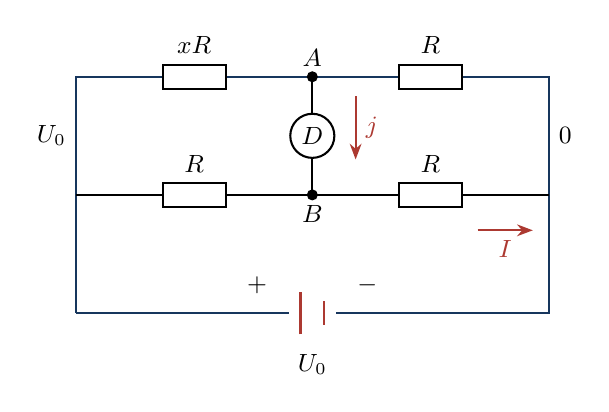
\begin{tikzpicture}
\draw[main] (0,0)--(0,3)--(6,3)--(6,0)--(0,0);
\draw (0,1.5)--(6,1.5);\draw (3,1.5)--(3,3);
\foreach \x/\y/\lab in {1.5/3/xR,4.5/3/R,1.5/1.5/R,4.5/1.5/R}{\fill[white] (\x-.4,\y-.15) rectangle (\x+.4,\y+.15);\draw (\x-.4,\y-.15) rectangle (\x+.4,\y+.15);\node[above] at (\x,\y+.16){$\lab$};}
\fill[white] (3,2.25) circle (.28);\draw (3,2.25) circle (.28);\node at (3,2.25){$D$};
\fill[white] (2.7,-.3) rectangle (3.3,.3);\draw[accent,very thick] (2.85,-.27)--(2.85,.27);\draw[accent,thick] (3.15,-.15)--(3.15,.15);\node[below] at (3,-.4){$U_0$};\node at (2.3,.35){$+$};\node at (3.7,.35){$-$};
\fill (3,3) circle (2pt);\fill (3,1.5) circle (2pt);\node[above] at (3,3){$A$};\node[below] at (3,1.5){$B$};
\draw[arr,accent] (5.1,1.05)--(5.8,1.05) node[midway,below]{$I$};\draw[arr,accent] (3.55,2.75)--(3.55,1.95) node[midway,right]{$j$};
\node[left] at (0,2.25){$U_0$};\node[right] at (6,2.25){$0$};
\end{tikzpicture}
\begin{tikzpicture}
\draw[main] (0,0)--(0,3)--(6,3)--(6,0)--(0,0);
\draw (0,1.5)--(6,1.5);\draw (3,1.5)--(3,3);
\foreach \x/\y/\lab in {1.5/3/xR,4.5/3/R,1.5/1.5/R,4.5/1.5/R}{\fill[white] (\x-.4,\y-.15) rectangle (\x+.4,\y+.15);\draw (\x-.4,\y-.15) rectangle (\x+.4,\y+.15);\node[above] at (\x,\y+.16){$\lab$};}
\fill[white] (3,2.25) circle (.28);\draw (3,2.25) circle (.28);\node at (3,2.25){$D$};
\fill[white] (2.7,-.3) rectangle (3.3,.3);\draw[accent,very thick] (2.85,-.27)--(2.85,.27);\draw[accent,thick] (3.15,-.15)--(3.15,.15);\node[below] at (3,-.4){$U_0$};\node at (2.3,.35){$+$};\node at (3.7,.35){$-$};
\fill (3,3) circle (2pt);\fill (3,1.5) circle (2pt);\node[above] at (3,3){$A$};\node[below] at (3,1.5){$B$};
\draw[arr,accent] (5.1,1.05)--(5.8,1.05) node[midway,below]{$I$};\draw[arr,accent] (3.55,2.75)--(3.55,1.95) node[midway,right]{$j$};
\node[left] at (0,2.25){$U_0$};\node[right] at (6,2.25){$0$};\node[note] at (3,-1.7){$V_B=IR$，$j=2I-U_0/R$\\$u=V_A-V_B=U_0-RI(3x+1)/(1+x)$};
\end{tikzpicture}
\begin{tikzpicture}
\draw[arr] (0,0)--(6.8,0) node[right]{$x$};
\draw[arr] (0,0)--(0,3.5) node[above]{$IR/U_0$};
\draw[main,thick] (0.00000,3.00000) -- (0.02500,2.86047) -- (0.05000,2.73913) -- (0.07500,2.63265) -- (0.10000,2.53846) -- (0.12500,2.45455) -- (0.15000,2.37931) -- (0.17500,2.31148) -- (0.20000,2.25000) -- (0.22500,2.19403) -- (0.25000,2.14286) -- (0.27500,2.09589) -- (0.30000,2.05263) -- (0.32500,2.01266) -- (0.35000,2.00000) -- (0.37500,2.00000) -- (0.40000,2.00000) -- (0.42500,2.00000) -- (0.45000,2.00000) -- (0.47500,2.00000) -- (0.50000,2.00000) -- (0.52500,2.00000) -- (0.55000,2.00000) -- (0.57500,2.00000) -- (0.60000,2.00000) -- (0.62500,2.00000) -- (0.65000,2.00000) -- (0.67500,2.00000) -- (0.70000,2.00000) -- (0.72500,2.00000) -- (0.75000,2.00000) -- (0.77500,2.00000) -- (0.80000,2.00000) -- (0.82500,2.00000) -- (0.85000,2.00000) -- (0.87500,2.00000) -- (0.90000,2.00000) -- (0.92500,2.00000) -- (0.95000,2.00000) -- (0.97500,2.00000) -- (1.00000,2.00000) -- (1.02500,2.00000) -- (1.05000,2.00000) -- (1.07500,2.00000) -- (1.10000,2.00000) -- (1.12500,2.00000) -- (1.15000,2.00000) -- (1.17500,2.00000) -- (1.20000,2.00000) -- (1.22500,2.00000) -- (1.25000,2.00000) -- (1.27500,2.00000) -- (1.30000,2.00000) -- (1.32500,2.00000) -- (1.35000,2.00000) -- (1.37500,2.00000) -- (1.40000,2.00000) -- (1.42500,2.00000) -- (1.45000,2.00000) -- (1.47500,2.00000) -- (1.50000,2.00000) -- (1.52500,2.00000) -- (1.55000,2.00000) -- (1.57500,2.00000) -- (1.60000,2.00000) -- (1.62500,2.00000) -- (1.65000,2.00000) -- (1.67500,2.00000) -- (1.70000,2.00000) -- (1.72500,2.00000) -- (1.75000,2.00000) -- (1.77500,2.00000) -- (1.80000,2.00000) -- (1.82500,2.00000) -- (1.85000,2.00000) -- (1.87500,2.00000) -- (1.90000,2.00000) -- (1.92500,2.00000) -- (1.95000,2.00000) -- (1.97500,2.00000) -- (2.00000,2.00000) -- (2.02500,2.00000) -- (2.05000,2.00000) -- (2.07500,2.00000) -- (2.10000,2.00000) -- (2.12500,2.00000) -- (2.15000,2.00000) -- (2.17500,2.00000) -- (2.20000,2.00000) -- (2.22500,2.00000) -- (2.25000,2.00000) -- (2.27500,2.00000) -- (2.30000,2.00000) -- (2.32500,2.00000) -- (2.35000,2.00000) -- (2.37500,2.00000) -- (2.40000,2.00000) -- (2.42500,2.00000) -- (2.45000,2.00000) -- (2.47500,2.00000) -- (2.50000,2.00000) -- (2.52500,2.00000) -- (2.55000,2.00000) -- (2.57500,2.00000) -- (2.60000,2.00000) -- (2.62500,2.00000) -- (2.65000,2.00000) -- (2.67500,2.00000) -- (2.70000,2.00000) -- (2.72500,2.00000) -- (2.75000,2.00000) -- (2.77500,2.00000) -- (2.80000,2.00000) -- (2.82500,2.00000) -- (2.85000,2.00000) -- (2.87500,2.00000) -- (2.90000,2.00000) -- (2.92500,2.00000) -- (2.95000,2.00000) -- (2.97500,2.00000) -- (3.00000,2.00000) -- (3.02500,1.99752) -- (3.05000,1.99507) -- (3.07500,1.99267) -- (3.10000,1.99029) -- (3.12500,1.98795) -- (3.15000,1.98565) -- (3.17500,1.98337) -- (3.20000,1.98113) -- (3.22500,1.97892) -- (3.25000,1.97674) -- (3.27500,1.97460) -- (3.30000,1.97248) -- (3.32500,1.97039) -- (3.35000,1.96833) -- (3.37500,1.96629) -- (3.40000,1.96429) -- (3.42500,1.96231) -- (3.45000,1.96035) -- (3.47500,1.95842) -- (3.50000,1.95652) -- (3.52500,1.95464) -- (3.55000,1.95279) -- (3.57500,1.95096) -- (3.60000,1.94915) -- (3.62500,1.94737) -- (3.65000,1.94561) -- (3.67500,1.94387) -- (3.70000,1.94215) -- (3.72500,1.94045) -- (3.75000,1.93878) -- (3.77500,1.93712) -- (3.80000,1.93548) -- (3.82500,1.93387) -- (3.85000,1.93227) -- (3.87500,1.93069) -- (3.90000,1.92913) -- (3.92500,1.92759) -- (3.95000,1.92607) -- (3.97500,1.92456) -- (4.00000,1.92308) -- (4.02500,1.92161) -- (4.05000,1.92015) -- (4.07500,1.91871) -- (4.10000,1.91729) -- (4.12500,1.91589) -- (4.15000,1.91450) -- (4.17500,1.91312) -- (4.20000,1.91176) -- (4.22500,1.91042) -- (4.25000,1.90909) -- (4.27500,1.90778) -- (4.30000,1.90647) -- (4.32500,1.90519) -- (4.35000,1.90391) -- (4.37500,1.90265) -- (4.40000,1.90141) -- (4.42500,1.90018) -- (4.45000,1.89895) -- (4.47500,1.89775) -- (4.50000,1.89655) -- (4.52500,1.89537) -- (4.55000,1.89420) -- (4.57500,1.89304) -- (4.60000,1.89189) -- (4.62500,1.89076) -- (4.65000,1.88963) -- (4.67500,1.88852) -- (4.70000,1.88742) -- (4.72500,1.88633) -- (4.75000,1.88525) -- (4.77500,1.88418) -- (4.80000,1.88312) -- (4.82500,1.88207) -- (4.85000,1.88103) -- (4.87500,1.88000) -- (4.90000,1.87898) -- (4.92500,1.87797) -- (4.95000,1.87697) -- (4.97500,1.87598) -- (5.00000,1.87500) -- (5.02500,1.87403) -- (5.05000,1.87307) -- (5.07500,1.87211) -- (5.10000,1.87117) -- (5.12500,1.87023) -- (5.15000,1.86930) -- (5.17500,1.86838) -- (5.20000,1.86747) -- (5.22500,1.86657) -- (5.25000,1.86567) -- (5.27500,1.86478) -- (5.30000,1.86391) -- (5.32500,1.86303) -- (5.35000,1.86217) -- (5.37500,1.86131) -- (5.40000,1.86047) -- (5.42500,1.85962) -- (5.45000,1.85879) -- (5.47500,1.85796) -- (5.50000,1.85714) -- (5.52500,1.85633) -- (5.55000,1.85552) -- (5.57500,1.85472) -- (5.60000,1.85393) -- (5.62500,1.85315) -- (5.65000,1.85237) -- (5.67500,1.85160) -- (5.70000,1.85083) -- (5.72500,1.85007) -- (5.75000,1.84932) -- (5.77500,1.84857) -- (5.80000,1.84783) -- (5.82500,1.84709) -- (5.85000,1.84636) -- (5.87500,1.84564) -- (5.90000,1.84492) -- (5.92500,1.84421) -- (5.95000,1.84350) -- (5.97500,1.84280) -- (6.00000,1.84211);
\draw[dashed] (.333,0)--(.333,2.4) (3,0)--(3,2.4);\node[below] at (.333,0){$1/3$};\node[below] at (3,0){$3$};\node[left] at (0,2){$1/2$};\node[note] at (3,-1.2){平台从 $x=1/3$ 到 $3$；$x=1$ 在平台内部};
\end{tikzpicture}
\begin{tikzpicture}
\draw[arr] (-3,0)--(3,0) node[right]{$u/U_0$};\draw[arr] (0,-1.9)--(0,3.7) node[above]{$jR/U_0$};
\draw[main,very thick] (-1.8,-1)--(-1.8,0)--(1.8,0)--(1.8,3);\draw[main,dashed] (-1.8,-1)--(-1.8,-1.7) (1.8,3)--(1.8,3.5);\draw[fill=white,main] (-1.8,-1) circle (2pt);
\node[below] at (-1.8,0){$-1/4$};\node[below] at (1.8,0){$1/4$};\node[right] at (1.8,3){$1/2$};\node[left] at (-1.8,-1){$-1/6$};\node[note] at (0,-2.9){实线：本次扫描覆盖；空心点：仅趋近的极限\\虚线：可选的理想钳位延长};
\end{tikzpicture}
\begin{tikzpicture}
\node[box] (n0) at (0,0) {测量变量\\$I(x)$};
\node[box] (n1) at (5,0) {节点转换\\$u(x),j(x)$};
\node[box] (n2) at (5,-2.3) {特性关系\\$j=0$ 或 $u=\pm U_0/4$};
\node[box] (n3) at (0,-2.3) {功率检查\\$P_D=uj\ge0$};
\draw[arr] (n0)--(n1);\draw[arr] (n1)--(n2);\draw[arr] (n2)--(n3);
\node[note] at (2.5,-4.1) {器件电流不是题给的下右支路电流；电压须取两节点之差};
\end{tikzpicture}
\end{document}
